\subsection{Events classification}

Given an intermittent device with a certain on-time duration ($d_{on}$), we can classify external events from the device perspective as follows:
\begin{itemize}
		\item \textit{Short events}---The event duration is shorter than the on-time of an intermittent device ($d_{on} < t_{on}$). This event can be (i) repetitive, i.e. the acoustic wave caused by a deformed gear tooth; or (ii) non-repetitive, i.e. single word command for a voice assistant.  

		\item \textit{Long events}---The event duration is much longer than the on-time of an intermittent device ($d_{on} > t_{on} $). These events can be (i) simple, such that capturing a small fraction of the event is sufficient to get all the information, i.e. vibration; or (ii) complex, such that capturing the entire event is required for correct interpretation, i.e. a command of several words to a voice assistant system. 
\end{itemize}

\subsection{Intermittent devices classifications}
Intermittent devices can be classified based on the relation between their on/off cycles and the occurrence of external events:  
\begin{itemize}
		\item An \textit{Event oblivious} intermittent device starts running once its energy buffer is full, regardless of the occurrence of an external event. In other words, the dispersion of the on-times of this type of intermittent devices is unaffected by the occurrence of external events. 
		\item An \textit{Event aware} intermittent device enters sleep mode once its buffer is full and upon the occurrence of an external event starts software execution. The power cycles of this type of intermittent devices tend to synchronize as their up times is triggered by an event.  

\end{itemize}

Events aware intermittent devices tend to have a longer effective on-time: the time needed to capture an event and save the data in memory.
%
%

%A fundamental limitation of intermittent devices are their inherent repeated absence. A natural way to combat this limitation is by grouping these tiny devices together and abstracting them as a single \emph{intermittent distributed system}. The collective on-time of these devices should approach continuous time as their number increases. However, the on-time and off-time of  distributed intermittent systems depend on the environment and the load. As such, we do not expect, for example, a linear relationship between the number of nodes and the overall on-time. 

%An intermittent device uses a capacitor (a buffer) to store energy and, usually, the capacitor has operational and shutdown thresholds (Figure\,\ref{fig:powerCycle}). 
The on-time evolution of a event-oblivious distributed intermittent system, as more nodes join, depends on the special diversity of its individual nodes.
%Depending on their spatial diversity, the nodes of a distributed intermittent system can experience the same energy harvesting conditions or not.
\subsection{Intermittent devices}
%
\begin{figure}
	\centering
		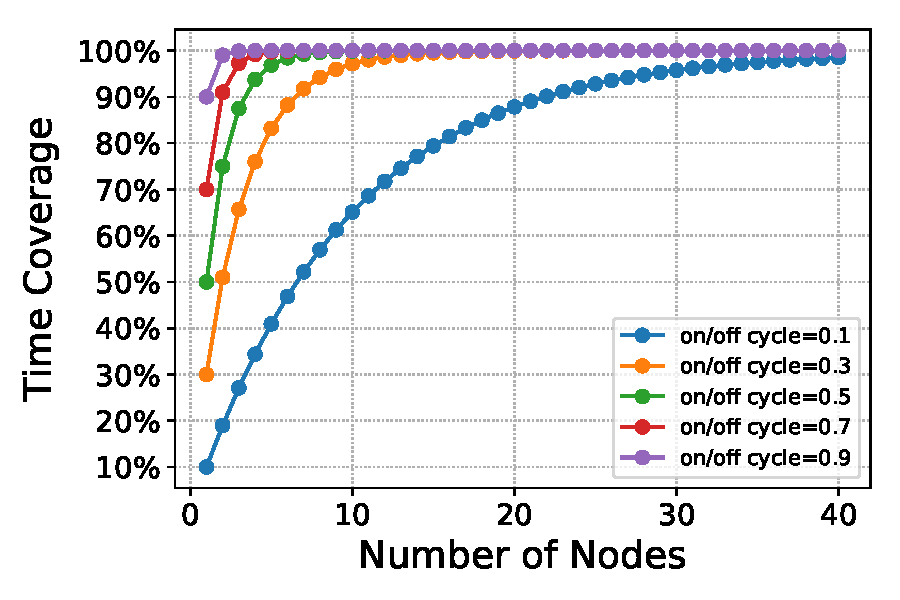
\includegraphics[width=\columnwidth]{figures/coverage.pdf}
	\caption{The on-time of a distributed intermittent system.}
	\label{fig:independentCoverage}
\end{figure}
%
\checkit{If the nodes are spatially diverse such that their energy harvesting rates are statistically different, then we can assume that the power cycles of the nodes are independent and uniformly distributed over the overall distributed system's power cycle}---When all the nodes power up and shutdown again\footnote{\todo{maybe it is better to define it as the mean of the individual power cycles}}. 
When the power cycles are uniformly distributed, adding a node increases the average on-time as follows, 
%
\begin{equation}
\delta t = \frac{t_{off}}{t_{sp}} * n_{on}
		\label{eq:indCov}
\end{equation}
%
where $t_{off}$ is the off-time of the distributed system, $t_{sp}$ is the period of the distributed system's power cycle, $n_{on}$ is a node on-time, and $\delta t$ is the time gain of the distributed intermittent system.

As Figure\,\ref{fig:independentCoverage} shows adding nodes to intermittent distributed systems increases its overall on-time, and consequently, its responsiveness. It is also clear that the benefit of an additional node is inversely proportional to the distributed system's on-time. Equation~\ref{eq:indCov}, however, holds only when nodes wake-ups approximate a uniform distribution. \checkit{When the nodes are in close proximity, we cannot model their power cycles as a random variable drawn from a uniform distribution because their energy charging rates are correlated}. 

%%
%\begin{figure}
%	\centering
%	\begin{subfigure}[t]{0.49\columnwidth}
%		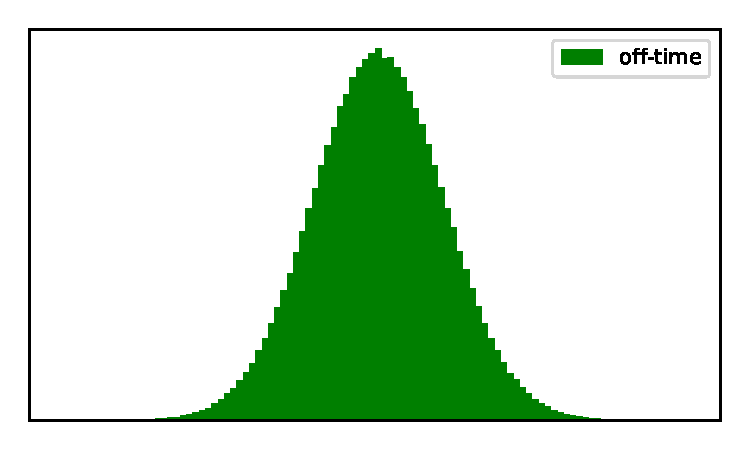
\includegraphics[width=\textwidth]{figures/offtime.pdf}
%			\caption{off-time length distribution}
%		\label{fig:offtime}
%	\end{subfigure}
%	\begin{subfigure}[t]{0.49\columnwidth}
%		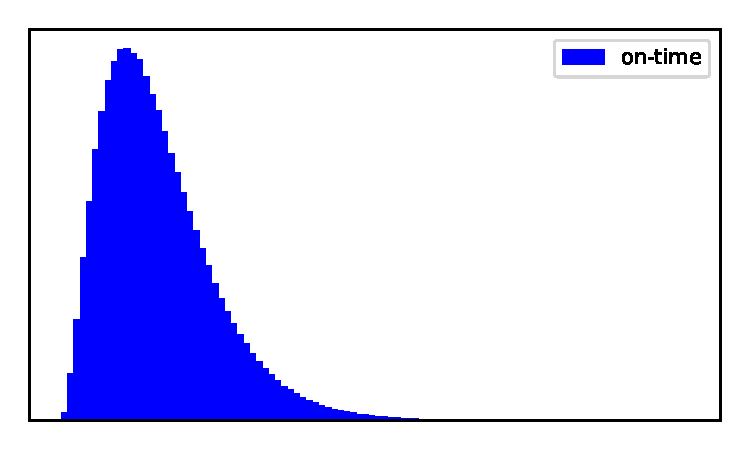
\includegraphics[width=\textwidth]{figures/ontime.pdf}
%		\caption{on-time length distribution}
%		\label{fig:ontime}
%	\end{subfigure}
%		\caption{The distributions of the operational stages of a distributed intermittent system.}		
%\end{figure}
%%

The \textit{off-time} of an intermittent device depends only on the environment: high charging rate results in short charging time and vice versa. Hence, we may model the off-time as a random variable drawn from a normal distribution (Figure\,\ref{fig:offtime}). The \textit{on-time}, however, depends on the buffered energy---the harvested energy while the device is off---; the harvested energy while the device is on, which only prolongs the execution; and the load of the device. Therefore, if we assume the load is constant, then we can model the on-time as a random variable drawn from a gamma distribution can be more appropriate (Figure\,\ref{fig:ontime}). Another important factor is \textit{the relation} between the off-time and the on-time. Short off-time indicates a high charging rate. A high harvesting rate results in a non-negligible amount of the harvested-while-executing energy. This energy lengthens the on-time. Therefore, we can conclude that there is an inverse relationship between the on-time and the off-time.

%
%To flatten the normal distribution we need to add another random variable that is drawn from a uniform-like distribution. To achieve that, we further randomize the length of the on-time of intermittent nodes by injecting delays---putting the nodes into sleep mode---upon devices' power-ups (Figure\,\ref{fig:spreading}). The maximum delay that can be added is bounded by the buffer size and the minimum energy consumption of the load. The length of this delay represents the spreading factor by which we spread the original distribution of the nodes' wake-ups.  
%
%\begin{figure}
%	\centering
%		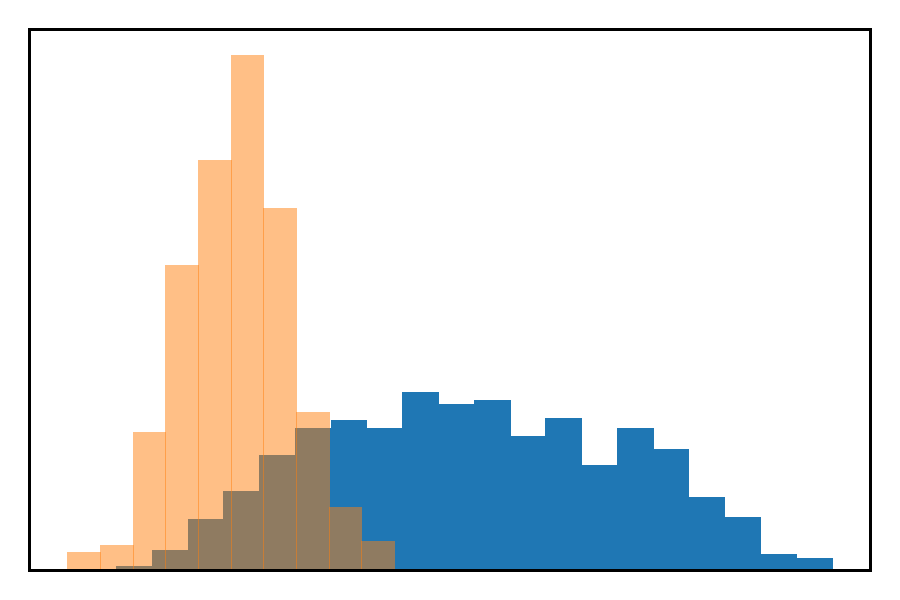
\includegraphics[width=\columnwidth]{figures/spreading.pdf}
%	\caption{Spreading normally distributed intermittent devices over a larger range by injecting delays with a uniformly distributed lengths.}
%	\label{fig:spreading}
%\end{figure}

%The energy charging rate is environment dependent, while the discharge rate is load dependent. If we assume ambient energy does not fluctuate very quickly, then we can conclude that there is an inverse relationship between the on-time (discharging time) and the off-time (charging time). Short charging time means fast energy shots arrival. High energy harvesting rate prolongs discharge (execution) time, as the device harvests a nonible amount of energy while executing. 



















